\section{Introduction}
\label{sec:introduction}

The following specification is broken down in to the core parts that describe the Zap wallet architecture. \\

\textbf{Predicate Wallet:}\

The predicate wallet (ZapWallet) is a stateless account abstraction wallet written in Sway for use on the Fuel network. The "wallet" is built from multiple
predicates called "Modules" and a "Master" predicate. Both the Master and Modules contain the logic to validate specific transaction
types signed by the owner of the wallet. The "Master" predicate is the asset holding address and serves
as the central point of validation control for ZapWallet transactions.\\

\textbf{Modules:}\

Modules in the ZapWallet architecture serve as specialized validation components that enable specific functionality while
maintaining the wallet's security. Each module validates specific types of transactions and have strict input, output and validation
criteria. A Module consists of the predicate code, a unique AssetId and a unique Address. \\

\textbf{Manager:}\

The manager contract (ZapManager) serves as a coordination point in the ZapWallet architecture, managing critical aspects of wallet
creation, operation and lifecycle. The ZapManager maintains three primary functions: \\

\textbf{1. Wallet Initialization.} The contract controls the initialization process for new ZapWallets by:
\begin{itemize}
    \item Minting and distributing initial nonce native assets required for new ZapWallets using Modules 1-3
    \item Managing associations between Ethereum addresses and their corresponding-ZapWallet
    \item Ensuring a ZapWallet can not re-initialize.
\end{itemize}

\textbf{2. Asset Management.} As the central authority for asset creation, the contract:
\begin{itemize}
    \item Acts as the sole minter for all module assets
    \item Controls nonce token creation and distribution
    \item Maintains integrity of module asset allocation
\end{itemize}

\textbf{3. Upgrade.} Controls the ability for version upgrades:
\begin{itemize}
    \item Verifies wallet ownership through nonce asset validation
    \item Manages phased transition from initialization to upgrade states
    \item Tracks upgrade status through module asset verification
    \item Maintains version pair numbering for both V1 and V2 wallet implementations
\end{itemize}


\subsection{ZapWallet Architecture}

The ZapWallet architecture consists of a master predicate that coordinates with multiple specialized module predicates,
as shown in Figure \ref{fig:zapwallet-structure}.

\begin{figure}[h]
    \centering
    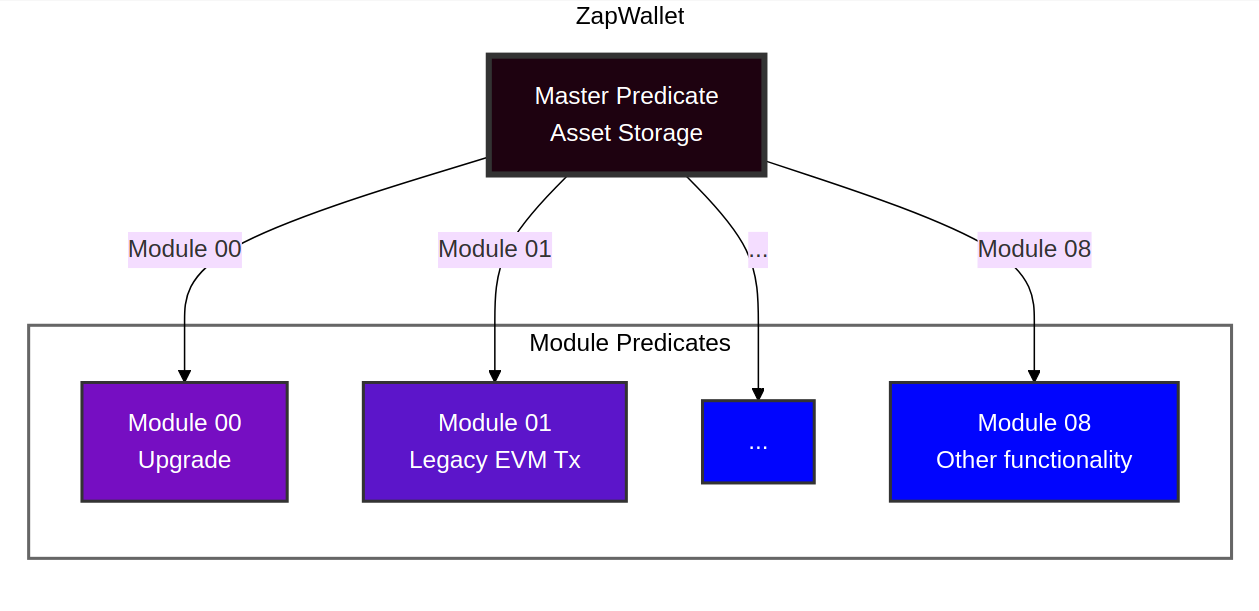
\includegraphics[width=0.9\textwidth]{images/architecture-structure2.png}
    \caption{ZapWallet Architectural Overview}
    \label{fig:zapwallet-structure}
\end{figure}

The Master predicate serves as the central authority for transactions and asset storage, while Modules provide specific functionality:

\begin{itemize}
    \item \textbf{Module 00 (Upgrade):} Handles wallet upgrade operations
    \item \textbf{Module 01 (Legacy EVM Tx):} Processes legacy Ethereum transactions (first-price auction model)
    \item \textbf{Module 02 (EIP-1559 EVM Tx):} Processes Ethereum EIP-1559 transactions (base fee + priority fee model) for Fuel \text{BASE\_ASSET} only
    \item \textbf{Module 03 (EIP-1559 EVM Tx):} Processes ERC20 style Ethereum EIP-1559 transactions (base fee + priority fee model) for Fuel native assets; SRC20 etc
    \item \textbf{Module 04 (TXID Witnessing):} Processes any type of Fuel transaction with the owner witnessing the transaction ID
    \item \textbf{Module 05 (Native Transfer):} Processes any Fuel native asset transaction (with the ability to have gas sponsorship) validated through a typed  data structure.
    \item \textbf{Module 06 (Not implemented):} Not implemented.
    \item \textbf{Module 07 (Gas Sponsor):} Supports gas sponsorship operations from an owners ZapWallet.
    \item \textbf{Module 08 (Not implemented):} Not implemented.
    \item Additional modules provide various other functionalities
    % \item \textbf{Module 08:} Extends wallet capabilities with specific features
\end{itemize}

Each module is identified by a unique AssetId and Address, ensuring secure and isolated operation.